\subsection{Additional figures and tables}

%%
% Table with details of the model fits
%
\begin{table}[!h]
  \centering

  \begin{subtable}{\linewidth}
    \centering
    \begin{tabular}{lllrrrr}
\toprule
{} & $t_0^{(2)}$ & $t^{(2)}_{N^{(2)}}$ & $f^{(1)}$ & $f^{(2)}$ & \emph{delta} & total uses \\
\midrule
MSNBC    &  2012-09-13 &          2012-09-27 &      2.03 &      3.19 &       0.57 &        283 \\
CNN      &  2012-11-07 &          2012-11-30 &      2.02 &      0.58 &      -0.71 &        213 \\
Fox News &  2012-09-09 &          2012-09-25 &      2.41 &      1.65 &      -0.31 &        262 \\
\bottomrule
\end{tabular}

    \caption{\quad2012; total uses: 758}
    \label{tab:fit-parameters-2012}
  \end{subtable}
  
  \vspace{.25in}

  \begin{subtable}{\linewidth}
    \centering
    \begin{tabular}{lllrrrr}
\toprule
  {} & $t_0^{(2)}$ & $t^{(2)}_{N^{(2)}}$ & $f^{(1)}$ & $f^{(2)}$ & \emph{delta} & total uses \\
\midrule
MSNBC    &  2016-10-08 &          2016-10-26 &      0.85 &      2.04 &       1.40 &        126 \\
CNN      &  2016-09-23 &          2016-10-27 &      1.14 &      2.81 &       1.45 &        196 \\
Fox News &  2016-09-23 &          2016-10-22 &      1.12 &      3.60 &       2.22 &        261 \\
\bottomrule
\end{tabular}

    \caption{\quad2016; total uses: 583}
    \label{tab:fit-parameters-2016}
  \end{subtable}

  \caption{Parameters for the best-fit (most likely) model for 2012 and 2016.}
  \label{tab:fit-parameters}
\end{table}

%%
% Table with network and violent words
%
\begin{table}[h]
  \centering

  \begin{subtable}{\linewidth}
    \centering
    \begin{tabular}{llrrrr}
\toprule
       &     & $f^{(1)}$ & $f^{(2)}$ & \emph{delta} & total uses \\
Violent Word & Network &           &           &            &            \\
\midrule
hit & MSNBC &      0.86 &      0.86 &      -0.00 &         67 \\
       & CNN &      0.54 &      0.11 &      -0.81 &         34 \\
       & Fox News &      0.57 &      0.33 &      -0.42 &         41 \\
\hline
beat & MSNBC &      1.03 &      1.64 &       0.59 &         89 \\
       & CNN &      0.66 &      0.63 &      -0.04 &         51 \\
       & Fox News &      0.83 &      0.53 &      -0.35 &         60 \\
\hline
attack & MSNBC &      1.30 &      3.14 &       1.42 &        127 \\
       & CNN &      2.07 &      0.32 &      -0.85 &        128 \\
       & Fox News &      2.08 &      2.00 &      -0.04 &        161 \\
\bottomrule
\end{tabular}

    \caption{\quad 2012}
    \label{tab:words-2012}
  \end{subtable}
  
  \vspace{.25in}

  \begin{subtable}{\linewidth}
    \centering
    \begin{tabular}{llrrrr}
\toprule
       &     & $f^{(1)}$ & $f^{(2)}$ & \emph{delta} & total uses \\
Violent Word & Network &           &           &            &            \\
\midrule
hit & MSNBC &      0.16 &      0.06 &      -0.63 &         10 \\
       & CNN &      0.27 &      0.45 &       0.64 &         25 \\
       & Fox News &      0.46 &      1.36 &       1.97 &         56 \\
\hline
beat & MSNBC &      0.54 &      1.47 &       1.75 &         55 \\
       & CNN &      0.50 &      0.79 &       0.59 &         45 \\
       & Fox News &      0.48 &      0.88 &       0.84 &         45 \\
\hline
attack & MSNBC &      0.61 &      1.59 &       1.62 &         61 \\
       & CNN &      1.16 &      2.59 &       1.23 &        126 \\
       & Fox News &      1.08 &      4.32 &       2.99 &        160 \\
\bottomrule
\end{tabular}

    \caption{\quad 2016}
    \label{tab:words-2016}
  \end{subtable}

  \caption{Uses and \emph{delta} for violence signals on each network in 2012 and 2016.}
  \label{tab:words}
\end{table}

% \begin{table}[!h]

%   \centering
%   \bgroup
%     \begin{subtable}{\textwidth}
%       \centering
%       \begin{tabular}{lr}
%         \toprule
%         Program name & Total MV uses \\
%         \midrule
%         The Rachel Maddow Show (MSNBC) & 93 \\
%         Hardball With Chris Matthews (MSNBC) & 208 \\
%         Anderson Cooper 360 (CNN) & 99 \\
%         Piers Morgan Tonight (CNN) & 118 \\
%         The O'Reilly Factor (Fox News) & 141 \\
%         Hannity (Fox News) & 133 \\
%         \bottomrule
%       \end{tabular}
%       \caption{Total uses by show in 2012}
%       \label{tab:by-show-2012}
%     \end{subtable} \\  \vspace{1.5em}
%     \begin{subtable}{\textwidth}
%       \centering
%       \begin{tabular}{lr}
%         \toprule
%         Program name & Total MV uses \\
%         \midrule
%         The Rachel Maddow Show (MSNBC) & 66 \\
%         The Last Word with Lawrence O'Donnel (MSNBC) & 80 \\
%         Anderson Cooper 360 (CNN) & 100 \\
%         Erin Burnett OutFront (CNN) & 118 \\
%         The O'Reilly Factor (Fox News) & 146 \\
%         The Kelly File (Fox News) & 148 \\
%         \bottomrule
%       \end{tabular} \quad
%       \caption{Total uses by show in 2016}
%       \label{tab:by-show-2016}
%     \end{subtable}

%   \egroup
%   \caption{Total uses by show in each of the two years}
%   \label{tab:by-show}
% \end{table}

\clearpage
\begin{figure}[!h]
  \centering
    \begin{subfigure}{0.9\linewidth}
      \centering
      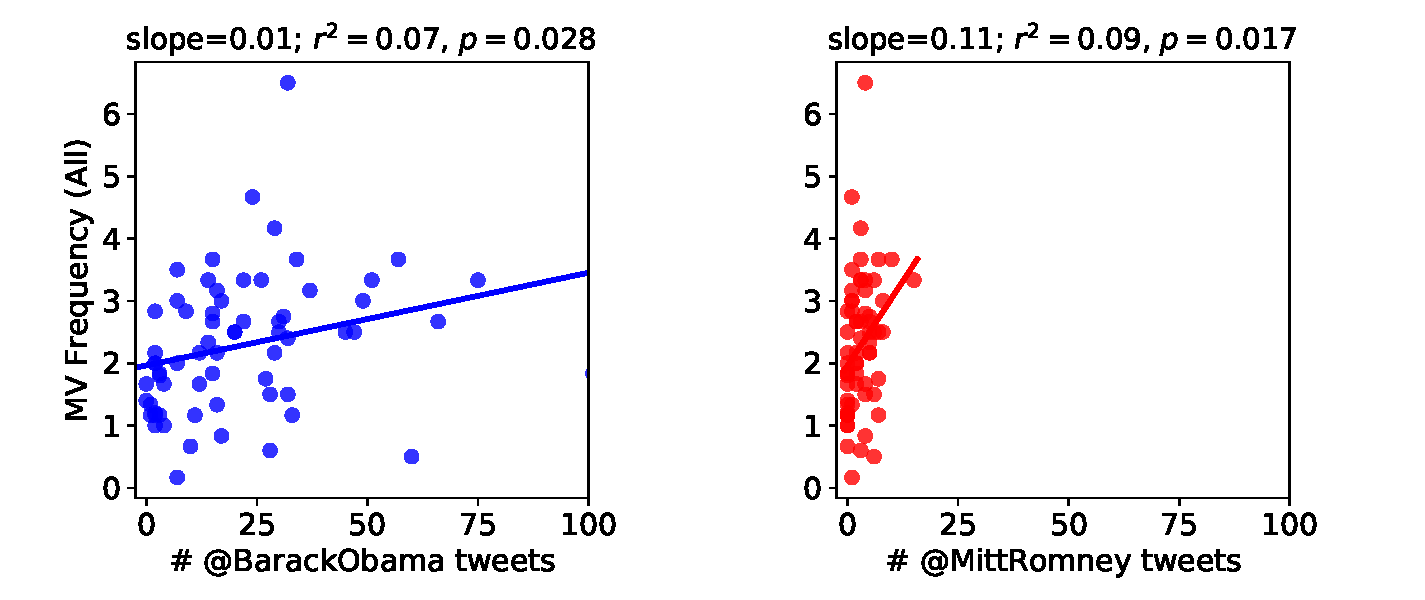
\includegraphics[width=\textwidth]{Figures/2012-all.pdf}
      \caption{2012}
      \label{fig:2012-all-reg}
    \end{subfigure} \\[2em]
    \begin{subfigure}{0.9\linewidth}
      \centering
      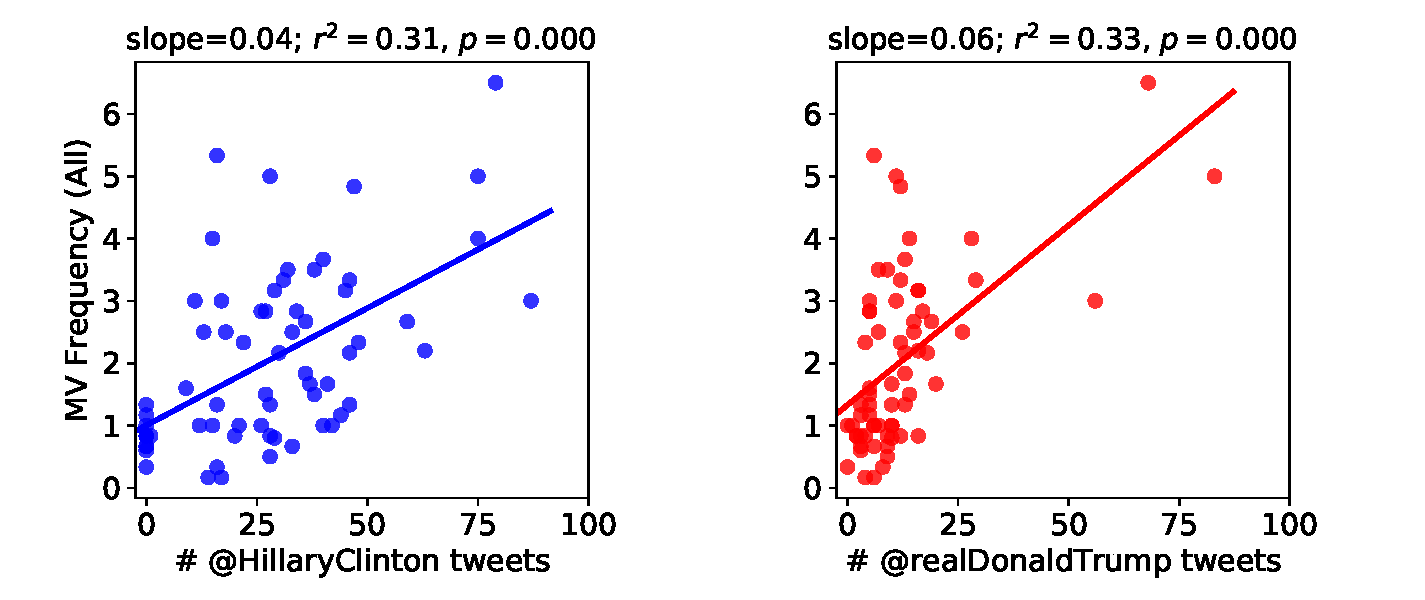
\includegraphics[width=\textwidth]{Figures/2016-all.pdf}
      \caption{2016}
      \label{fig:2012-all-reg}
    \end{subfigure}
  \caption{Metaphorical violence tracked candidate tweets significantly in 2012 and
    2016. Frequency is over all networks and subject/object relationships.
    Correlation coefficient is greater in 2016 than 2012, supporting other 
    claims of 2016 being a ``Twitter election.''
  }
  \label{fig:regressions-all}
\end{figure}

\clearpage

\begin{figure}[!h]
  \centering
    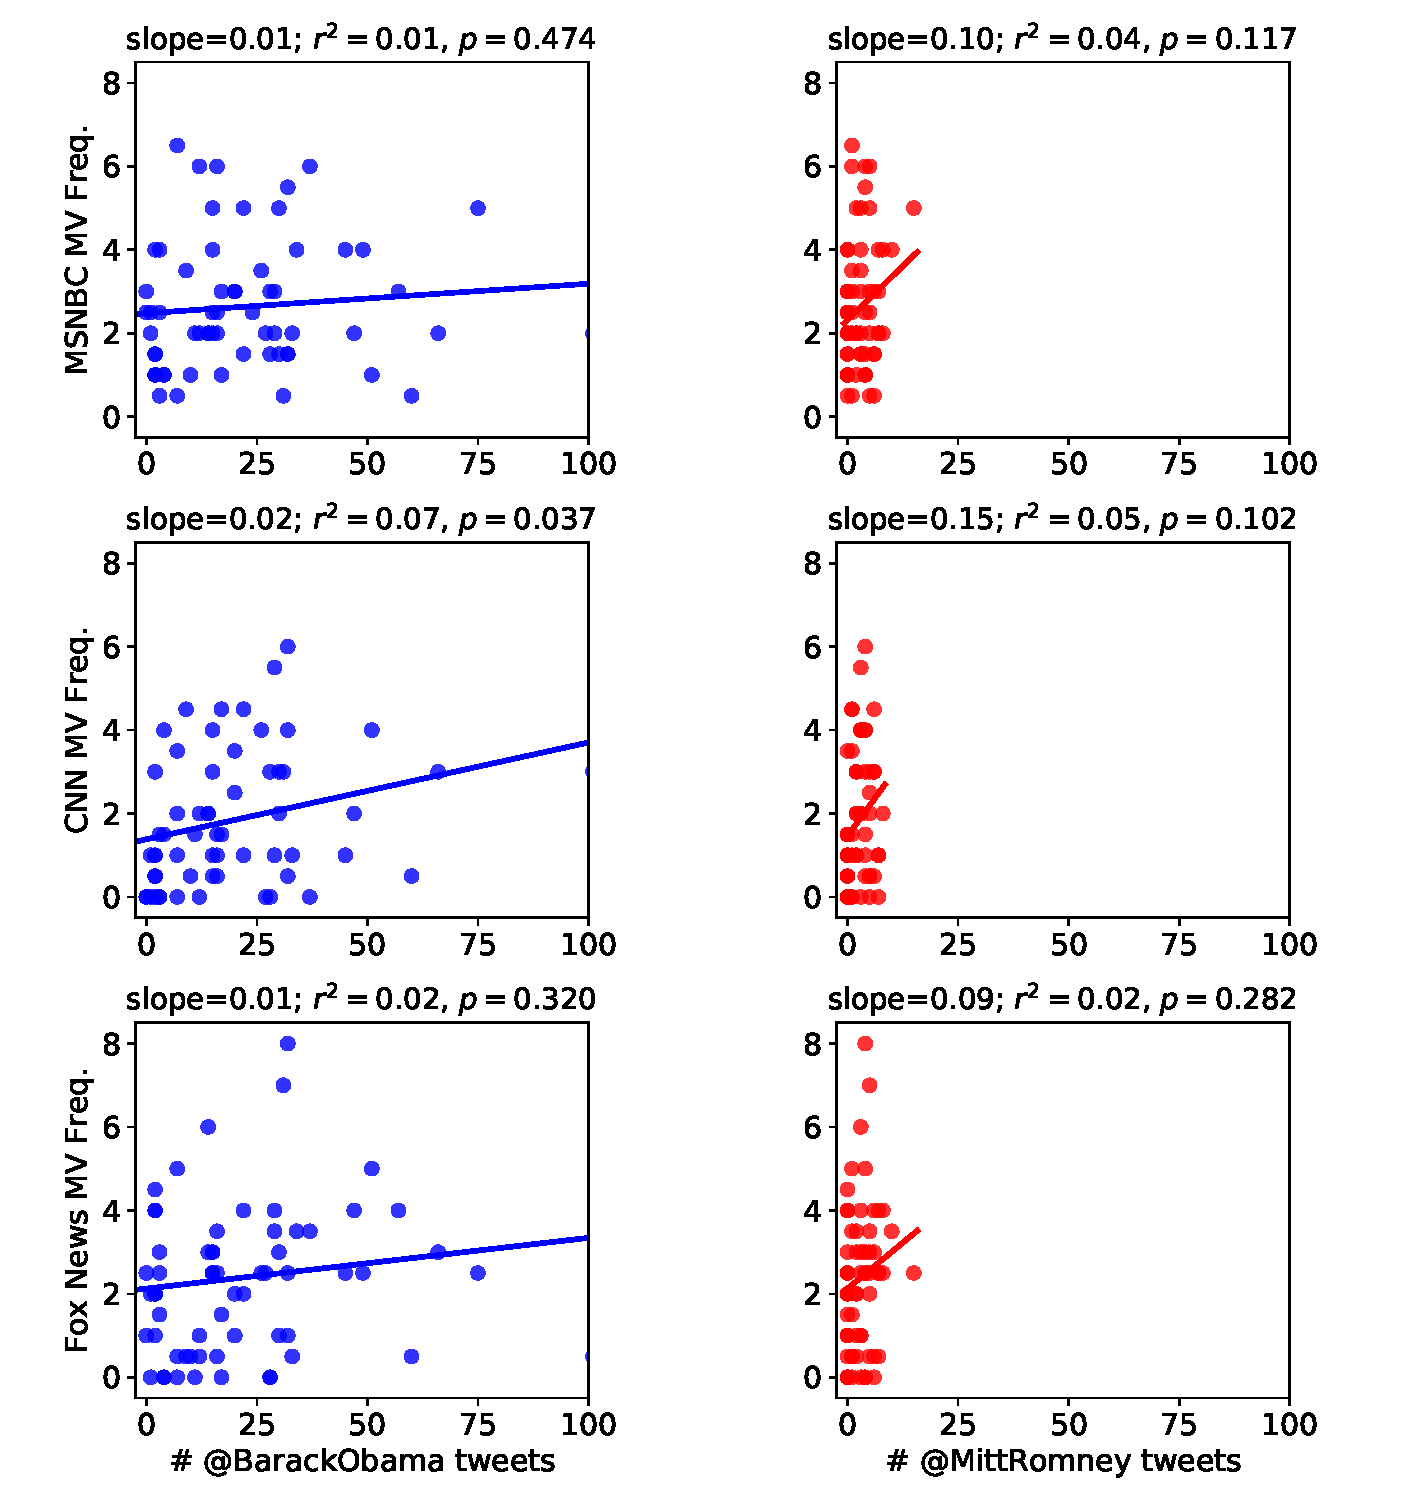
\includegraphics[width=0.95\textwidth]{Figures/2012-network.pdf}
  \caption{Regressions of metaphorical violence on each network in response
   to tweets from @BarackObama and @MittRomney.}
  \label{fig:2012-network}
\end{figure}


\begin{figure}[H]
  \centering
    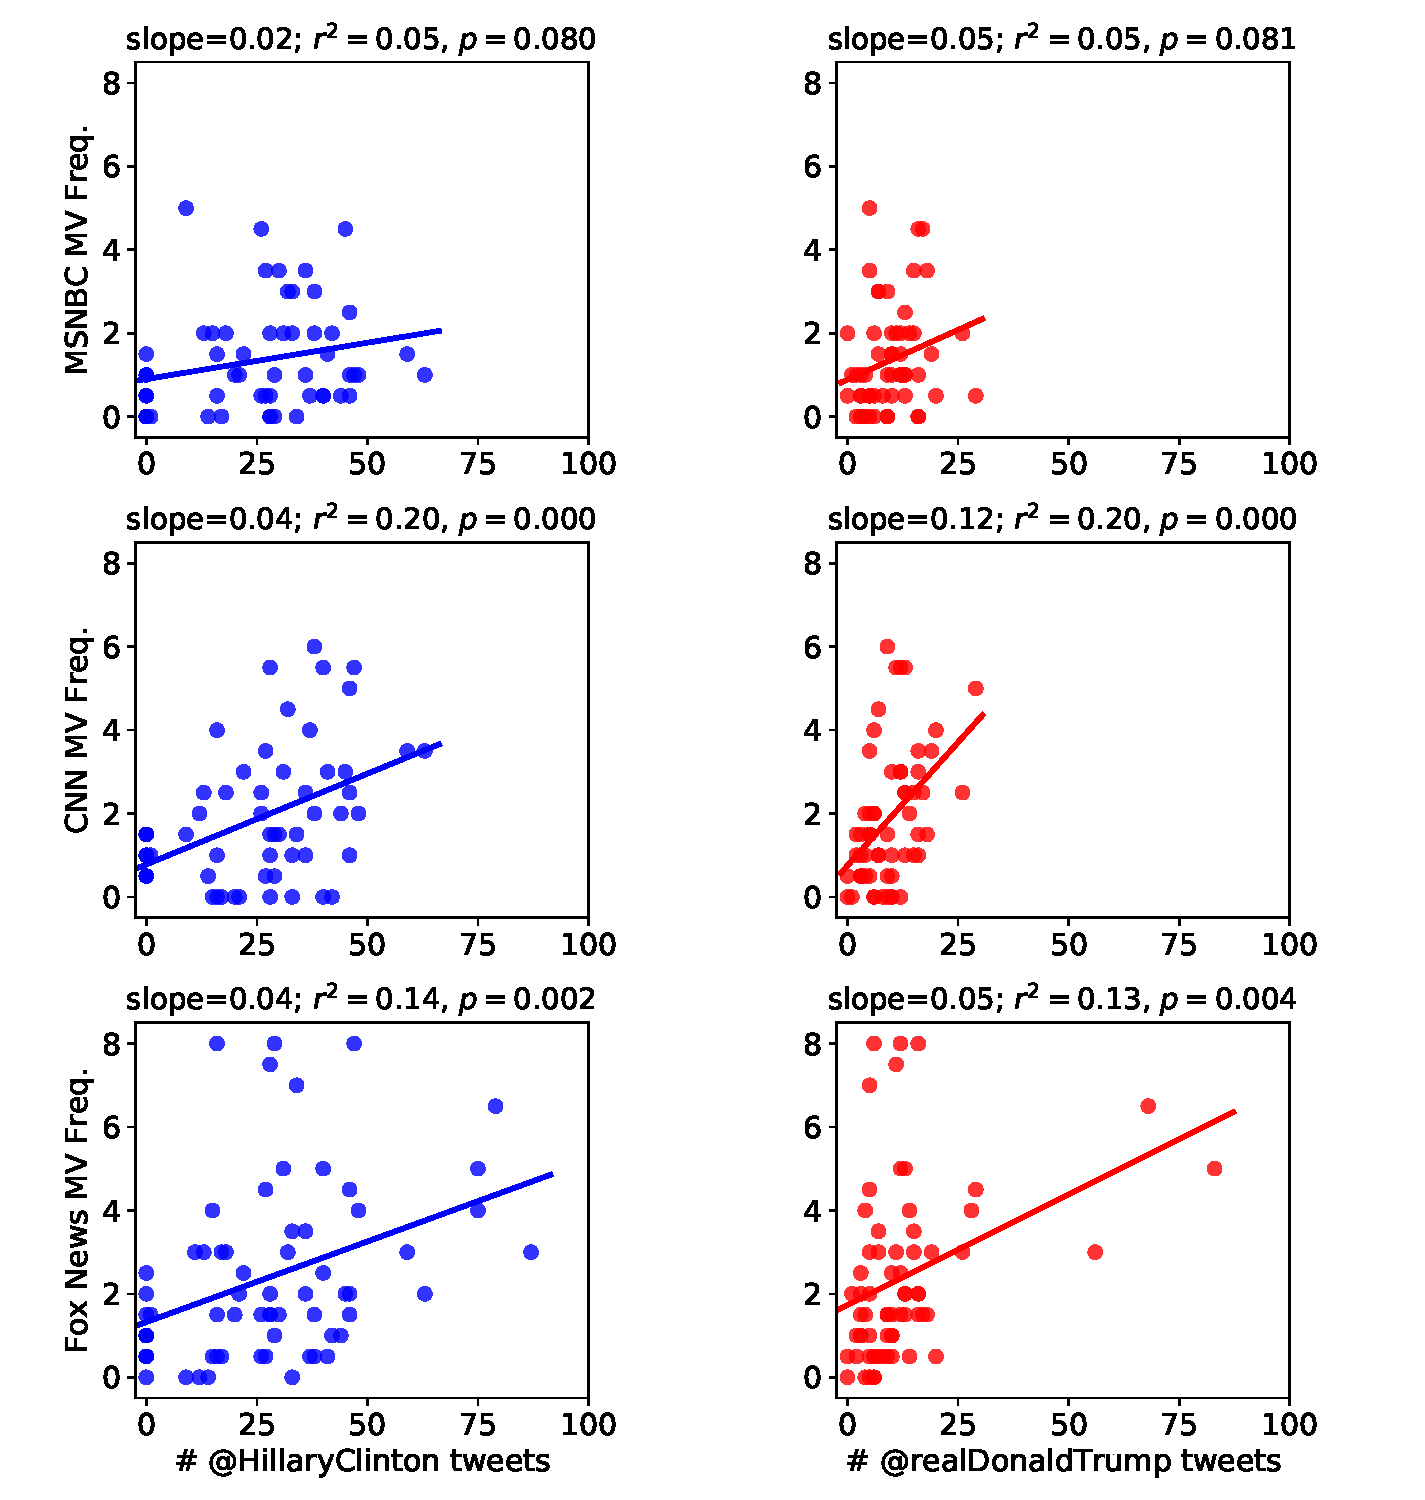
\includegraphics[width=0.95\textwidth]{Figures/2016-network.pdf}
  \caption{Regressions of metaphorical violence on each network in response
   to tweets from @HillaryClinton and @realDonaldTrump.}
  \label{fig:2016-network}
\end{figure}


\begin{figure}[H]
  \centering
    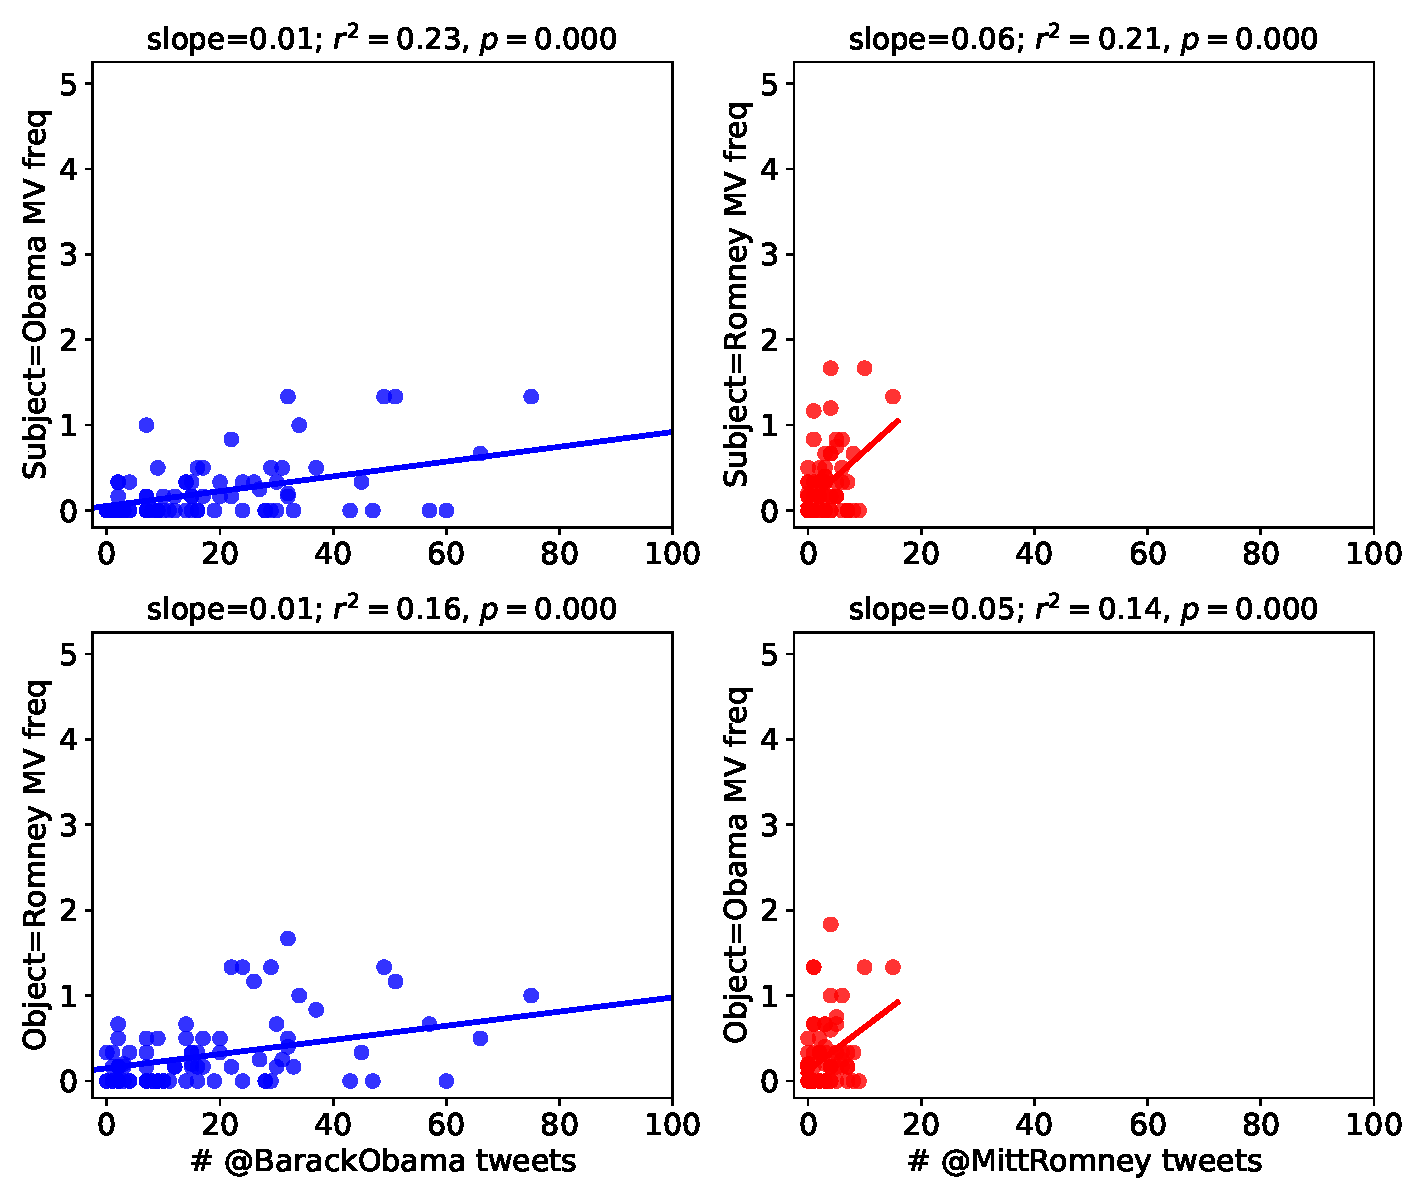
\includegraphics[width=0.9\textwidth]{Figures/2012-subjobj.pdf}
  \caption{Regressions of metaphorical violence faceted by subject and object
    in response to to tweets from @BarackObama and @MittRomney.}
  \label{fig:2012-subjobj}
\end{figure}


\begin{figure}[H]
  \centering
    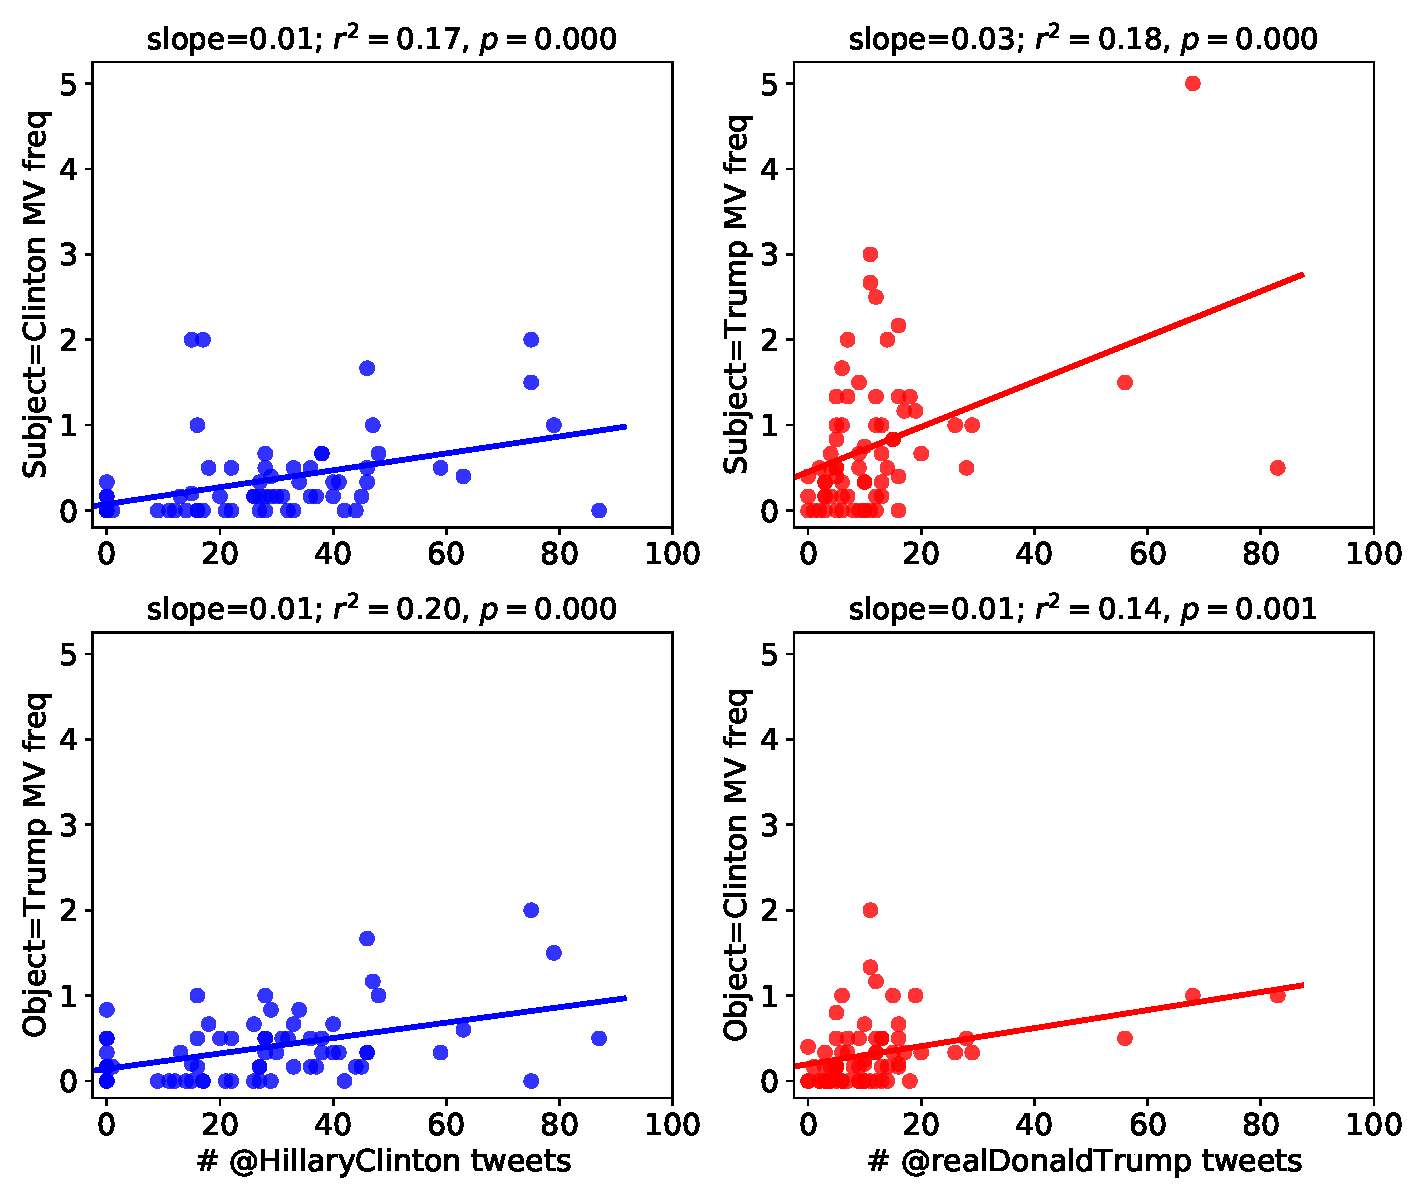
\includegraphics[width=0.9\textwidth]{Figures/2016-subjobj.pdf}
  \caption{Regressions of metaphorical violence faceted by subject and object
    in response to to tweets from @HillaryClinton and @realDonaldTrump.}
  \label{fig:2016-subjobj}
\end{figure}

\clearpage

\subsection{Notes on model fitting}

We presented both Bayesian-type relative likelihood inference probabilities
for the fitted models as well as the frequntist p-value measure for each 
candidate model parameterization. Frequentists can breathe a sigh of relief, 
since all but one model's optimal paramaterization had a p-value greater than
0.01; it was 0.011. The other five optimal models had p-value significance 
less than 0.01 (Tables~\ref{tab:relative-likelihoods-2012} 
and~\ref{tab:relative-likelihoods-2016}).  While the significance can
tell us whether or not a model is appropriate for the data, there were many 
models that were significant from a frequentist perspective. The relative
likelihood of alternative parameterizations tells us the probability that an
alternative parameterization will capture more information about the dynamics
than the parameterization with minimal AIC, our chosen information metric.
In an inexact sense, the various relative likelihoods tell us the weight of
each parameterization in some superordinate representation that is a
weighted sum of all potential parameterizations. Exactly this is done in some
applications, where a weighted sum of models is selected as the optimal model, 
typically models with a differing number of independent dimensions.
The presence of either greater or fewer large relative likelihoods signals either
a stronger or weaker presence of the impulse-type behavior we have hypothesized.
In 2012, the presence of an impulse was much weaker, with the next nine most
likely parameterizations having a relative likelihood greater than 0.5, with
two exceptions of .47 and .41 for MSNBC (Table~\ref{tab:supp-msnbc-2012}). 
In 2016, only one alternative had a relative
likelihood greater than 0.5, also on MSNBC: 0.508 
(Table~\ref{tab:supp-msnbc-2016}). So in this sense, MSNBC had the best-defined
impulse in 2012 and the worst-defined impulse in 2016.

In 2012, two networks showed negative reactivity.
In one case, CNN's MV usage dips after election
day, perhaps there was no longer a cultural driving force for MV usage
because there was no more ``fighting'' in the debates or elections. 
The other case where
reactivity was negative was Fox News' MV usage in 2012. This may be because
Obama was perceived as the more skilled debater and the Republican side 
avoided raising emotions and expectations over the debates, or other reasons
discussed later. MSNBC showed positive reactivity in 2012, 
more than doubling its frequency from its initial base level to its 
modulated level.  In 2016, the three networks showed greater coherence in their 
behavior.  Fox News was the most reactive, followed closely by CNN. The time period
of Fox News' modulated state lasted ten days longer than CNN's. MSNBC was 
the least reactive, but with a significant reactivity of 163\% 
(Table~\ref{tab:fit-parameters}).




\begin{table}[!h]
  \centering

  \bgroup
    \begin{subtable}{\linewidth}
      % \hfill
      \centering
      \begin{tabular}{rllrr}
\toprule
 rel. lik. & $t_0^{(2)}$ & $t^{(2)}_{N^{(2)}}$ & reactivity &  $P(<|t|)$ \\
\midrule
  1.000000 &  2012-09-12 &          2012-09-26 &       0.94 &   0.000326 \\
  0.951229 &  2012-09-09 &          2012-09-26 &       0.90 &   0.000344 \\
  0.582086 &  2012-09-09 &          2012-09-27 &       0.85 &   0.000572 \\
  0.565037 &  2012-09-12 &          2012-09-27 &       0.88 &   0.000590 \\
  0.506725 &  2012-09-10 &          2012-10-17 &       0.79 &   0.000660 \\
  0.431549 &  2012-09-10 &          2012-10-18 &       0.79 &   0.000780 \\
  0.397452 &  2012-09-09 &          2012-10-04 &       0.77 &   0.000850 \\
  0.379520 &  2012-09-10 &          2012-09-28 &       0.81 &   0.000892 \\
  0.354267 &  2012-09-10 &          2012-10-16 &       0.76 &   0.000959 \\
  0.346991 &  2012-09-12 &          2012-09-28 &       0.83 &   0.000980 \\
\bottomrule
\end{tabular}

      \caption{MSNBC; 2012}
      \label{tab:supp-msnbc-2012}
    \end{subtable} \\  \vspace{1.5em}

    \begin{subtable}{\linewidth}
      \centering
      \begin{tabular}{rllrr}
\toprule
 rel. lik. & $t_0^{(2)}$ & $t^{(2)}_{N^{(2)}}$ & reactivity &  $P(<|t|)$ \\
\midrule
  1.000000 &  2012-11-06 &          2012-11-29 &      -0.70 &   0.000148 \\
  0.875496 &  2012-10-26 &          2012-11-29 &      -0.61 &   0.000170 \\
  0.772116 &  2012-11-07 &          2012-11-29 &      -0.71 &   0.000193 \\
  0.607375 &  2012-11-08 &          2012-11-30 &      -0.72 &   0.000247 \\
  0.514332 &  2012-11-06 &          2012-11-28 &      -0.70 &   0.000293 \\
  0.427936 &  2012-10-30 &          2012-11-30 &      -0.60 &   0.000354 \\
  0.405132 &  2012-11-07 &          2012-11-28 &      -0.70 &   0.000375 \\
  0.375951 &  2012-10-02 &          2012-10-15 &       1.18 &   0.000405 \\
  0.352062 &  2012-09-27 &          2012-10-15 &       1.08 &   0.000433 \\
  0.324736 &  2012-11-08 &          2012-11-28 &      -0.71 &   0.000471 \\
\bottomrule
\end{tabular}
  
      \caption{CNN; 2012}
        \label{tab:supp-cnn-2012}
    \end{subtable} \\  \vspace{1.5em}

    \begin{subtable}{\linewidth}
      \centering
      \begin{tabular}{rllrr}
\toprule
 rel. lik. & $t_0^{(2)}$ & $t^{(2)}_{N^{(2)}}$ & reactivity &  $P(<|t|)$ \\
\midrule
  1.000000 &  2012-09-12 &          2012-09-24 &      -0.55 &   0.025549 \\
  0.917421 &  2012-09-11 &          2012-09-24 &      -0.52 &   0.028131 \\
  0.860348 &  2012-09-09 &          2012-09-24 &      -0.50 &   0.030230 \\
  0.820812 &  2012-09-07 &          2012-09-24 &      -0.48 &   0.031871 \\
  0.646732 &  2012-09-11 &          2012-09-23 &      -0.51 &   0.041741 \\
  0.614601 &  2012-09-07 &          2012-11-20 &      -0.36 &   0.044240 \\
  0.607754 &  2012-09-10 &          2012-09-23 &      -0.48 &   0.044810 \\
  0.583962 &  2012-09-08 &          2012-11-26 &      -0.42 &   0.046906 \\
  0.581079 &  2012-09-07 &          2012-09-22 &      -0.46 &   0.047173 \\
  0.507553 &  2012-09-25 &          2012-10-06 &       0.54 &   0.055126 \\
\bottomrule
\end{tabular}
 
      \caption{Fox News; 2012}
      \label{tab:supp-fox-2012}
    \end{subtable}
  \egroup

  \caption{Relative likelihood of the null model and the ten most-likely
    dynamical models with alternative parameterizations. Parameterizations given
    are the first and last date of the excited state.}
  \label{tab:relative-likelihoods-2012}
\end{table}

\begin{table}[!h]
  \centering
  \bgroup
    \begin{subtable}{\linewidth}
      % \hfill
      \centering
      \begin{tabular}{rllrr}
\toprule
 rel. lik. & $t_0^{(2)}$ & $t^{(2)}_{N^{(2)}}$ & reactivity &  $P(<|t|)$ \\
\midrule
  1.000000 &  2016-10-08 &          2016-10-26 &       1.40 &   0.000015 \\
  0.385238 &  2016-10-08 &          2016-10-25 &       1.34 &   0.000039 \\
  0.338263 &  2016-10-08 &          2016-11-03 &       1.28 &   0.000044 \\
  0.220983 &  2016-10-06 &          2016-10-26 &       1.26 &   0.000068 \\
  0.158223 &  2016-10-11 &          2016-10-26 &       1.29 &   0.000096 \\
  0.158223 &  2016-10-10 &          2016-10-25 &       1.29 &   0.000096 \\
  0.158002 &  2016-10-08 &          2016-11-05 &       1.21 &   0.000096 \\
  0.126735 &  2016-10-09 &          2016-11-03 &       1.19 &   0.000120 \\
  0.115298 &  2016-10-07 &          2016-11-03 &       1.18 &   0.000132 \\
  0.114875 &  2016-10-08 &          2016-11-06 &       1.19 &   0.000133 \\
\bottomrule
\end{tabular}

      \caption{MSNBC; 2016}
      \label{tab:supp-msnbc-2016}
    \end{subtable} \\  \vspace{1.5em}

    \begin{subtable}{\linewidth}
      \centering
      \begin{tabular}{rllrr}
\toprule
 rel. lik. & $t_0^{(2)}$ & $t^{(2)}_{N^{(2)}}$ & reactivity &  $P(<|t|)$ \\
\midrule
  1.000000 &  2016-09-25 &          2016-10-27 &       1.45 &   0.000073 \\
  0.764196 &  2016-09-24 &          2016-11-04 &       1.55 &   0.000095 \\
  0.760063 &  2016-09-25 &          2016-10-13 &       1.46 &   0.000096 \\
  0.661919 &  2016-09-25 &          2016-11-03 &       1.50 &   0.000110 \\
  0.654467 &  2016-09-27 &          2016-10-27 &       1.40 &   0.000112 \\
  0.648921 &  2016-09-26 &          2016-10-13 &       1.46 &   0.000113 \\
  0.537424 &  2016-09-23 &          2016-10-20 &       1.37 &   0.000136 \\
  0.450599 &  2016-09-26 &          2016-11-04 &       1.45 &   0.000163 \\
  0.399820 &  2016-09-26 &          2016-11-03 &       1.41 &   0.000184 \\
  0.398737 &  2016-09-23 &          2016-10-12 &       1.41 &   0.000185 \\
\bottomrule
\end{tabular}
  
      \caption{CNN; 2016}
        \label{tab:supp-cnn-2016}
    \end{subtable} \\  \vspace{1.5em}

    \begin{subtable}{\linewidth}
      \centering
      \begin{tabular}{rllrr}
\toprule
 rel. lik. & $t_0^{(2)}$ & $t^{(2)}_{N^{(2)}}$ & reactivity &     $P(<|t|)$ \\
\midrule
  1.000000 &  2016-09-24 &          2016-10-22 &       2.22 &  1.991356e-11 \\
  0.270536 &  2016-09-23 &          2016-10-24 &       2.17 &  7.238780e-11 \\
  0.041894 &  2016-09-25 &          2016-10-25 &       2.08 &  4.577034e-10 \\
  0.031166 &  2016-09-22 &          2016-10-23 &       2.03 &  6.134216e-10 \\
  0.019854 &  2016-09-23 &          2016-10-21 &       1.96 &  9.586853e-10 \\
  0.015325 &  2016-09-23 &          2016-10-26 &       2.05 &  1.239016e-09 \\
  0.012477 &  2016-09-16 &          2016-10-23 &       2.20 &  1.518961e-09 \\
  0.011004 &  2016-09-21 &          2016-10-23 &       1.99 &  1.720502e-09 \\
  0.006018 &  2016-09-16 &          2016-10-24 &       2.19 &  3.130088e-09 \\
  0.004315 &  2016-09-21 &          2016-10-24 &       1.95 &  4.354356e-09 \\
\bottomrule
\end{tabular}
 
      \caption{Fox News; 2016}
      \label{tab:supp-fox-2016}
    \end{subtable}
  \egroup

  \caption{Relative likelihood of the null model and the ten most-likely
    dynamical models with alternative parameterizations. Parameterizations given
    are the first and last date of the excited state.}
  \label{tab:relative-likelihoods-2016}
\end{table}

